\documentclass{beamer}

\usepackage{helvet}
\usepackage{hyperref, graphicx}
\usepackage{amsthm}
\usepackage{etoolbox}
\usepackage{multicol}
\usepackage{caption}

\usetheme[progressbar=frametitle, numbering=none]{metropolis}
\usecolortheme[snowy]{owl}
\setbeamertemplate{navigation symbols}{}
\AtBeginSection[ ]
{
\begin{frame}{Outline}
    \tableofcontents[currentsection]
\end{frame}
}

% Default fixed font does not support bold face
\DeclareFixedFont{\ttb}{T1}{txtt}{bx}{n}{11} % for bold
\DeclareFixedFont{\ttm}{T1}{txtt}{m}{n}{12}  % for normal - use in headings

% Custom colors
\usepackage{color}
\definecolor{TUGray}{RGB}{101,101,137}
\definecolor{TUBlack}{RGB}{0,0,10}
\definecolor{mygreen}{RGB}{45,111,63}
\definecolor{keywords}{RGB}{205,114,0}
\definecolor{comments}{RGB}{181,51,139}
\definecolor{strings}{RGB}{58,144,81}
\definecolor{numeric}{RGB}{66,110,176}
\definecolor{linos}{rgb}{0.4,0.4,0.4}
\definecolor{links}{rgb}{0,0.4,0.75}

\definecolor{bggray}{RGB}{232, 233, 235}

\setbeamercolor{alerted text}{fg=mygreen}
\setbeamercolor{normal text}{fg=TUBlack}\usebeamercolor*{normal text}

\setbeamercolor{codecol}{fg=TUGray!25!black,bg=bggray}

\hypersetup{colorlinks, linkcolor=links, urlcolor=links}

\usepackage[T1]{fontenc}
\usepackage[sfdefault,scaled=.85]{FiraSans}
%\usepackage{newtxsf}
\usepackage{mathpazo}

\usepackage{listings}

\newtoggle{InString}{}% Keep track of if we are within a string
\togglefalse{InString}% Assume not initally in string

\newcommand\digitstyle{\color{numeric}}
\makeatletter
\newcommand{\ProcessDigit}[1]
{%
  \ifnum\lst@mode=\lst@Pmode\relax%
   {\digitstyle #1}%
  \else
    #1%
  \fi
}
\makeatother

\lstset{literate=%
    {0}{{{\ProcessDigit{0}}}}1
    {1}{{{\ProcessDigit{1}}}}1
    {2}{{{\ProcessDigit{2}}}}1
    {3}{{{\ProcessDigit{3}}}}1
    {4}{{{\ProcessDigit{4}}}}1
    {5}{{{\ProcessDigit{5}}}}1
    {6}{{{\ProcessDigit{6}}}}1
    {7}{{{\ProcessDigit{7}}}}1
    {8}{{{\ProcessDigit{8}}}}1
    {9}{{{\ProcessDigit{9}}}}1
	{<=}{{\(\leq\)}}1
	{>=}{{\(\geq\)}}1,
	% morestring=[b]",
    % morestring=[b]',
    % morecomment=[l]{//},
}

\lstdefinelanguage{Pseudo}{
    morekeywords={begin, end, return, while},
    morecomment=[l]{\#},
}

% Pseudocode style
\newcommand\pseudostyle{\lstset{
language=Pseudo,
basicstyle=\fontfamily{ccr}\scriptsize,
commentstyle=\it\scriptsize\color{linos},
keywordstyle=\it\bfseries\scriptsize,
mathescape=true,
literate=
    {=}{$\leftarrow{}$}{1}
    {==}{$={}$}{1},
xleftmargin=18pt,
xrightmargin=4pt,
aboveskip=12pt,
belowskip=0pt,
frame=tB,
keepspaces=true
}}

% Python style for highlighting
\newcommand\pythonstyle{\lstset{
language=Python,
basicstyle=\ttfamily\tiny,
numbers=left,
numberstyle=\tiny\color{linos},
morekeywords={self, np},              % Add keywords here
keywordstyle=\tiny\color{keywords},
commentstyle=\it\tiny\color{comments},    % Custom highlighting style
stringstyle=\tiny\color{strings},
xleftmargin=18pt,
xrightmargin=4pt,
aboveskip=0pt,
belowskip=0pt,
escapeinside={(*@}{@*)},
frame=l,                         % Any extra options here
showstringspaces=false,
keepspaces=true
}}

% Pseudocode environment
\lstnewenvironment{pseudo}[1][]
{
    \pseudostyle
    \lstset{
        #1
    }
}
{}

% Python environment 
\lstnewenvironment{python}[1][]
{
	\pythonstyle
	\lstset{
	#1
	}
}
{}

% wrap the Python environment
\newenvironment{codeblock}
    {\hfill\begin{beamerboxesrounded}[lower=codecol, width=0.8\textwidth]
    \medskip

    }
    { 
    \end{beamerboxesrounded}\hfill
    }

\theoremstyle{example}
\newtheorem{question}{Question}

\newcommand{\ct}[1]{\lstinline[language=Python,basicstyle=\ttfamily\footnotesize,stringstyle=\small\color{strings}]!#1!}
\newcommand{\ttt}[1]{{\small\texttt{#1}}}
\newcommand{\lsitem}[2]{\ttt{{#1}[}\ct{#2}\ttt{]}}
\newcommand{\bb}[1]{\mathbb{#1}}
\newcommand{\cl}[1]{\mathcal{#1}}
\newcommand{\comment}[1]{}

\author{Chris Cornwell}
\date{September 11, 2025}
\title{Linear regression through Optimization}

\begin{document}

\begin{frame}
\titlepage
\end{frame}

\begin{frame}
\frametitle{Outline}
\tableofcontents
\end{frame}

\section{Generalizing Linear regression to multiple variables}

\begin{frame}{Extending the linear regression procedure}
    If you have data $({\bf x}_1,y_1), ({\bf x}_2,y_2), \ldots, ({\bf x}_P, y_P)$ where, for some $N>1$ the input ${\bf x}_i$ is a vector in $\bb R^N$, can you still do linear regression?

    \pause
    For each $i$ with $1\le i\le P$, say that ${\bf x}_i = {\scriptsize \begin{bmatrix}x_{1,i}\\ x_{2,i}\\ \vdots\\ x_{N,i}\end{bmatrix}}$. Define a $P\times(N+1)$ matrix $A$ so that the $i^{th}$ row is $[1, x_{1,i}, x_{2,i}, \ldots, x_{N,i}]$.\pause \newline 
    In other words, set $\tilde{\bf x}_i$ equal to the vector in $\bb R^{N+1}$ with $1$ as its first component and ${\bf x}_i$ for the remaining $N$ components. Then 
        \[A = \begin{bmatrix} \overset{\rule{0.4cm}{0.02cm}}{\phantom{.}} & \tilde{\bf x}_1^T & \overset{\rule{0.4cm}{0.02cm}}{\phantom{.}} \\ \overset{\rule{0.4cm}{0.02cm}}{\phantom{.}} & \tilde{\bf x}_2^T & \overset{\rule{0.4cm}{0.02cm}}{\phantom{.}} \\ & \vdots & \\ \overset{\rule{0.4cm}{0.02cm}}{\phantom{.}} & \tilde{\bf x}_P^T & \overset{\rule{0.4cm}{0.02cm}}{\phantom{.}} \end{bmatrix}.\]
\end{frame}

\begin{frame}{Extending the linear regression procedure}
    A solution $\tilde{\bf w}^\star = [b^\star, w_1^\star, \ldots, w_N^\star]^T$ to the normal equations $A^TA\tilde{\bf w} = A^T{\bf y}$ (with $A$ as above) gives coefficients for a linear model for the data.\footnote{\small The matrix $A^TA$ is $(N+1)\times(N+1)$ and $A^T{\bf y}$ is a vector in $\bb R^{N+1}$.}

    \vspace*{-2pt}
    \pause
    Write ${\bf w}^\star \in \bb R^{N}$ for the non-constant coefficient vector ${\scriptsize [w_1^\star,w_2^\star,\ldots,w_N^\star]^T}$. The affine linear model on the data, in $N$ variables, is \vspace*{-4pt} 
    \[f_{\tilde{\bf w}^\star}({\bf x}) = b^\star + w_1^\star x_1 + \ldots + w_N^\star x_N = b^\star + {\bf x}^T{\bf w}^\star.\] 

    \vspace*{-15pt}   
    \begin{enumerate}
        \pause
        \item[(1)] $f_{\tilde{\bf w}^\star}({\bf x})$ is affine linear, meaning the difference in two function values is a dot product on the difference of the input. Specifically, $f_{\tilde{\bf w}^\star}({\bf x}) - f_{\tilde{\bf w}^\star}({\bf x}') = ({\bf x} - {\bf x}')^T{\bf w}^\star$.
        \pause
        \item[(2)] The graph of $f_{\tilde{\bf w}^\star}({\bf x})$ is a hyperplane\footnote{\small Generalization of a plane in $\bb R^3$.} in $\bb R^{N+1}$ with normal vector ${\scriptsize [1,-w_1^\star, \ldots, -w_N^\star]^T}$.
    \end{enumerate}
    \vfill
\end{frame}

\begin{frame}{Example}
    \textbf{A concrete example:} using the data in \ct{'Advertising.csv'}, found in the \href{https://github.com/cornwell/math371-S25/blob/main/DataSets/}{DataSets folder} of the course site. \newline 
    This contains data on amounts spent (in thousands of dollars) on TV, Radio, and Newspaper advertising in 200 different markets, as well as the amounts sold in each market (in thousands of units).
    
    \pause
    \begin{multicols}{2}
    To perform linear regression, with independent variables \ct{'TV'}, \ct{'Radio'}, and \ct{'Newspaper'} and setting $y$ equal to \ct{'Sales'}, one may follow the procedure above. The matrix $A$ described is $200\times 4$ ($N=3$).\pause\ The resulting coefficients are (approximately) \[{\scriptsize [b^\star, w_1^\star, w_2^\star, w_3^\star] = [2.9389, 0.0458, 0.1885, -0.001].}\]
    
    \begin{figure}[tight]
    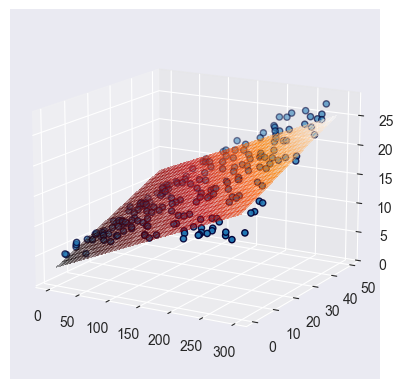
\includegraphics[width=0.3\textwidth]{../../Images/multiregression-higherangle.png}
    \caption*{{\footnotesize 3D projection of\\ Advertising model}}
    \end{figure}
    \end{multicols}
\end{frame}

\section{Measuring the fitness of linear models}

\begin{frame}{``Noise'' and linear regression model}
    \textbf{Underlying assumption:} the (input) variables $x_1,\ldots,x_N$ are not random, but there is natural variability in the ``$y$-direction'' (value of $f_{\tilde{\bf w}}$), represented with a random variable. \newline 
    For some $b$ and some ${\bf w} = [w_1,\ldots, w_N]^T$, 
    \[y = b + {\bf x}^T{\bf w} + \varepsilon\]
\end{frame}

\begin{frame}
    \frametitle{Least Squares loss function}
    On given data $({\bf x}_1, y_1), ({\bf x}_2, y_2), \ldots, ({\bf x}_P, y_P)$, the measure that is commonly used for how well a linear regression model, $f_{b,{\bf w}}({\bf x}) = b + {\bf x}^T{\bf w}$, fits the data is the Least Squares loss (cost) function. 
    \vspace*{-8pt}
    \begin{itemize}
        \item \textit{This is $P$ times the Mean Squared Error.}
    \end{itemize}

    Following notation from textbook, this loss function is 
        \[g(b, {\bf w}) = \sum_{p=1}^P\left(f_{b,{\bf w}}({\bf x}_p) - y_p\right)^2.\]
    
    %\centering 
    % 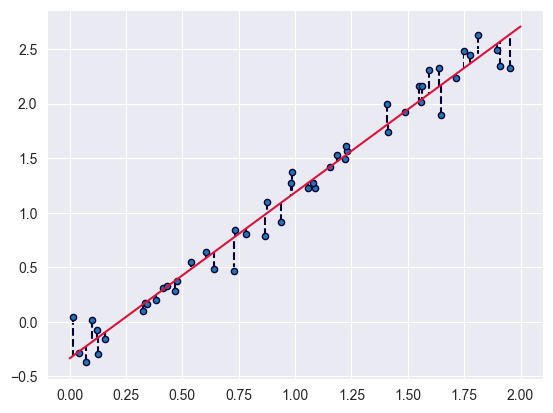
\includegraphics[width=0.4\textwidth]{lsr-error-lines.png}
\end{frame}

\begin{frame}
    \frametitle{Meaning of Least Squares loss}
    For $1\le p\le P$, since $f_{b,{\bf w}}({\bf x}_p) = \hat{y}_p$, the quantity $|f_{b,{\bf w}}({\bf x}_p) - y_p|$ is the vertical distance from $(x_p, y_p)$ to the point predicted by the linear model, $(x_p, \hat{y}_p)$. 

    Additionally, the length of the vector ${\bf y} - \hat{\bf y}$ (which is the distance from ${\bf y}$ to the point determined by $\tilde{\bf w}$, in the column space of our feature matrix) is equal to 
        \[\sqrt{(\hat{y}_1 - y_1)^2 + (\hat{y}_2 - y_2)^2 + \ldots + (\hat{y}_P - y_P)^2} = \sqrt{g(b, {\bf w})}.\]

    We see that minimizing $g(b, {\bf w})$ is the same as minimizing that distance, which will give us the $\hat{\bf y}$ in the column space that makes ${\bf y} - \hat{\bf y}$ be orthogonal to the column space.
\end{frame}

\begin{frame}
    \frametitle{Minimizing the Least Squares loss}
    The data $\{({\bf x}_p, y_p)\}_{p=1}^P$ is fixed. How do we solve the problem 
                \[\underset{\text{minimize}}{b,{\bf w}} g(b, {\bf w})?\]
    We can use methods from calculus, specifically the first order condition {--} that we want all partial derivatives equal to zero. 
    \begin{itemize}
        \item Note, what are the variables of the function $g$?  They are the parameters $b,w_1,w_2,\ldots,w_N$.
    \end{itemize}
    \vfill
    \pause
    Next: a review of calculus minimization techniques.
\end{frame}

\end{document}